\chapter{Test Results \label{6}}
After PCB was designed and successfully manufactured, it must be tested.
This chapter will include test methods and verification of the PDU hardware batch for the Descartes mission.
\\
Needed tools:\\ \\
$\bullet$ ESD-bracelet\\
$\bullet$ ESD-mat\\
$\bullet$ Power supply\\
$\bullet$ Oscilloscope\\
$\bullet$ Multimeter\\
$\bullet$ CubeMX\\
$\bullet$ Ac6 (Firmware to program STM32)\\
$\bullet$ Logic analyzer\\
$\bullet$ Test results excel sheet\\
$\bullet$ Bread board\\
$\bullet$ Electrical Load\\



\section{Resistance and Connectivity Check }


Resistance check is the first test for the PCB. This test needed to detect the shorts on the PCB before applying the power.
Every connectors pin of the PCB shall be measured with respect to the GND by using multimeter. As an expected result, multimeter shall show the constant measurement value.

Resistance check was completed flawlessly without any shorts. The test results is not shown in Master Thesis. 

Connectivity check needed to verify the top level requirements: TL19, TL20, TL21, TL22 from Chapter \ref{cha:chapter3}, Tab.\ref{Tab:req1} which required to provide a data signals to the payloads.


\captionof{table}{Connectivity check of the payload data lines}
\begin{center}
	

	\begin{tabular}{p{3cm}p{3cm}p{2cm}} \toprule
		
	Payload & Type of signal & Result \\ \midrule
	AURA & CAN & Pass\\
	AMUR & UART & Pass\\  
	DeCor & CAN & Pass\\
	LoRa & CAN & Pass\\
	\bottomrule
\end{tabular}\\ 

\end{center}
\label{Tab:connectivity}
Tab.\ref{Tab:connectivity} verifies the uppermention requirements.
\section{Switches}
This is a big section which includes the switches functionality such as enable/disable power output check, over-current feedback from the fault pins for every load switch  and the shift register control. \\
\\
Power switches work on 5 power lines:\\ \\
$\bullet$ 3.3V BUS\\
$\bullet$ 5V BUS\\
$\bullet$ 3.3V PAYL\\
$\bullet$ 5V PAYL\\
$\bullet$ 7.4V\\ \\
Enable pins of a power switches might be activated manually by providing a 3.3V to an appropriate enable pin or applying a enable signal from a microcontroller.  Six enable signals VCC 4, VCC 5, VCC 6, VCC 7, VCC 18 and VCC 19 have to be triggered by I$^2$C protocol via shift register.

On the Fig.\ref{fig: pdu_test_front}  and \ref{fig: pdu_test_back} illustrated switches and their pins, which needed to test power switches.



\begin{figure}[h]
	\centering
	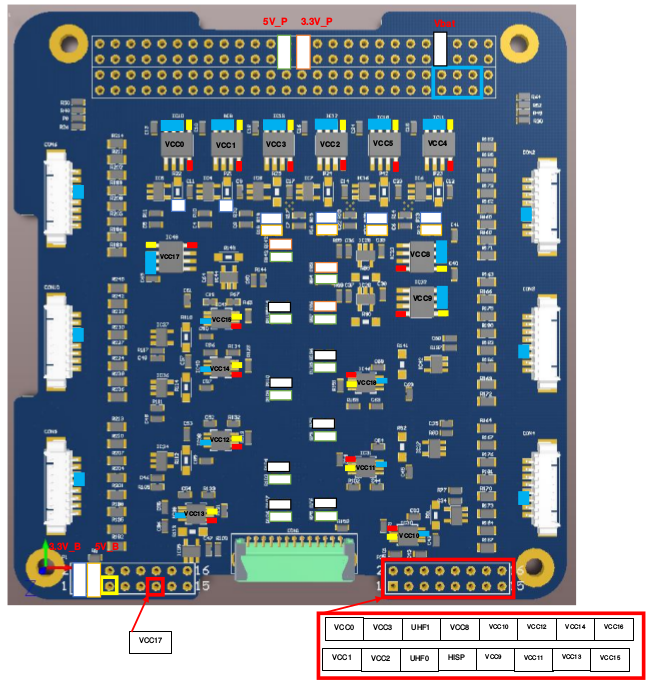
\includegraphics[scale=0.37]{pdu_front_test.png}
	\caption{Top view of the switch control}
	\label{fig: pdu_test_front}
\end{figure} 

\begin{figure}[h]
	\centering
	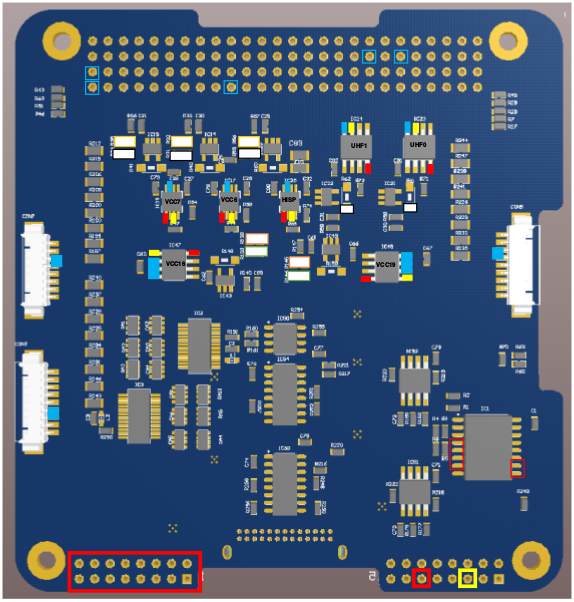
\includegraphics[scale=0.5]{pdu_bot_test.png}
	\caption{Bottom view of the switch control}
	\label{fig: pdu_test_back}
\end{figure}

STEPS:\\
\textbf{1.}  First of all, PDU has to be connected to the power source (PSU) which is adjusted to needed voltage.\\ \\
\textbf{2.} After power was supplied to the PDU, input voltage has to be checked. Figure \ref{fig: pdu_test_front} and Figure \ref{fig: pdu_test_back} illustrate the zero ohm resistors which connect the power line into the load switch. Voltage measure of the resistor can be done via multimeter. \\ \\
\textbf{3.} Shift register is initially turned on by default. To check shift register functionality it is necessary to provide an I$^2$C signal with a bit array to a shift register, which might be possible by using microcontroller (in my case STM32 L073Rz was used). Section \ref{shiftty} describes the work principles of the shift register in detail. In addition, test code for the sift register is given in the appendix. \\ \\
\textbf{4.} Check every output power line by providing enable signal according test file. This step can be done in two ways: providing a 3.3v from the PSU to enable connector or providing
enable signals to the PDU by using STM32 L073Rz, providing an enable signal using push button interrupt). As a result, switch has to transfer the power of the channel.\\ \\
\textbf{5.} Next step is to use the electrical load to simulate the subsystem an the payload load for the required channels.\\ \\
\textbf{6.} Over-current check has to be checked by connecting electrical load to the output power line
pin. Electrical load has to be adjusted in the way that power consumption of the line has to exceed the current
threshold of the switch. $\overline{OC}$ pin is expected to become low.
It is also important to know, that $\overline{OC}$ pin will show LOW if switch TPS1H200A does not have a load while it is enabled. If shift register does not turned off, $\overline{OC}$ will appear while 5V BUS and Vbat line is available.\\ \\
\textbf{7.} The next test is a maximum current check, the point of this test is to check the maximum current limit of all microchips, that were programmed for a
specific current limit, maximum current draw has to be simulated by electrical load. When current surpasses the expected
limit, $\overline{OC}$ pin will become LOW.
Fig.\ref{fig: pdu_test_front} and \ref{fig: pdu_test_back} illustrates the switches and its signals such as Vout (blue), Overcurrent (yellow), Enable (red).

 \begin{figure}[h]
 	\centering
 	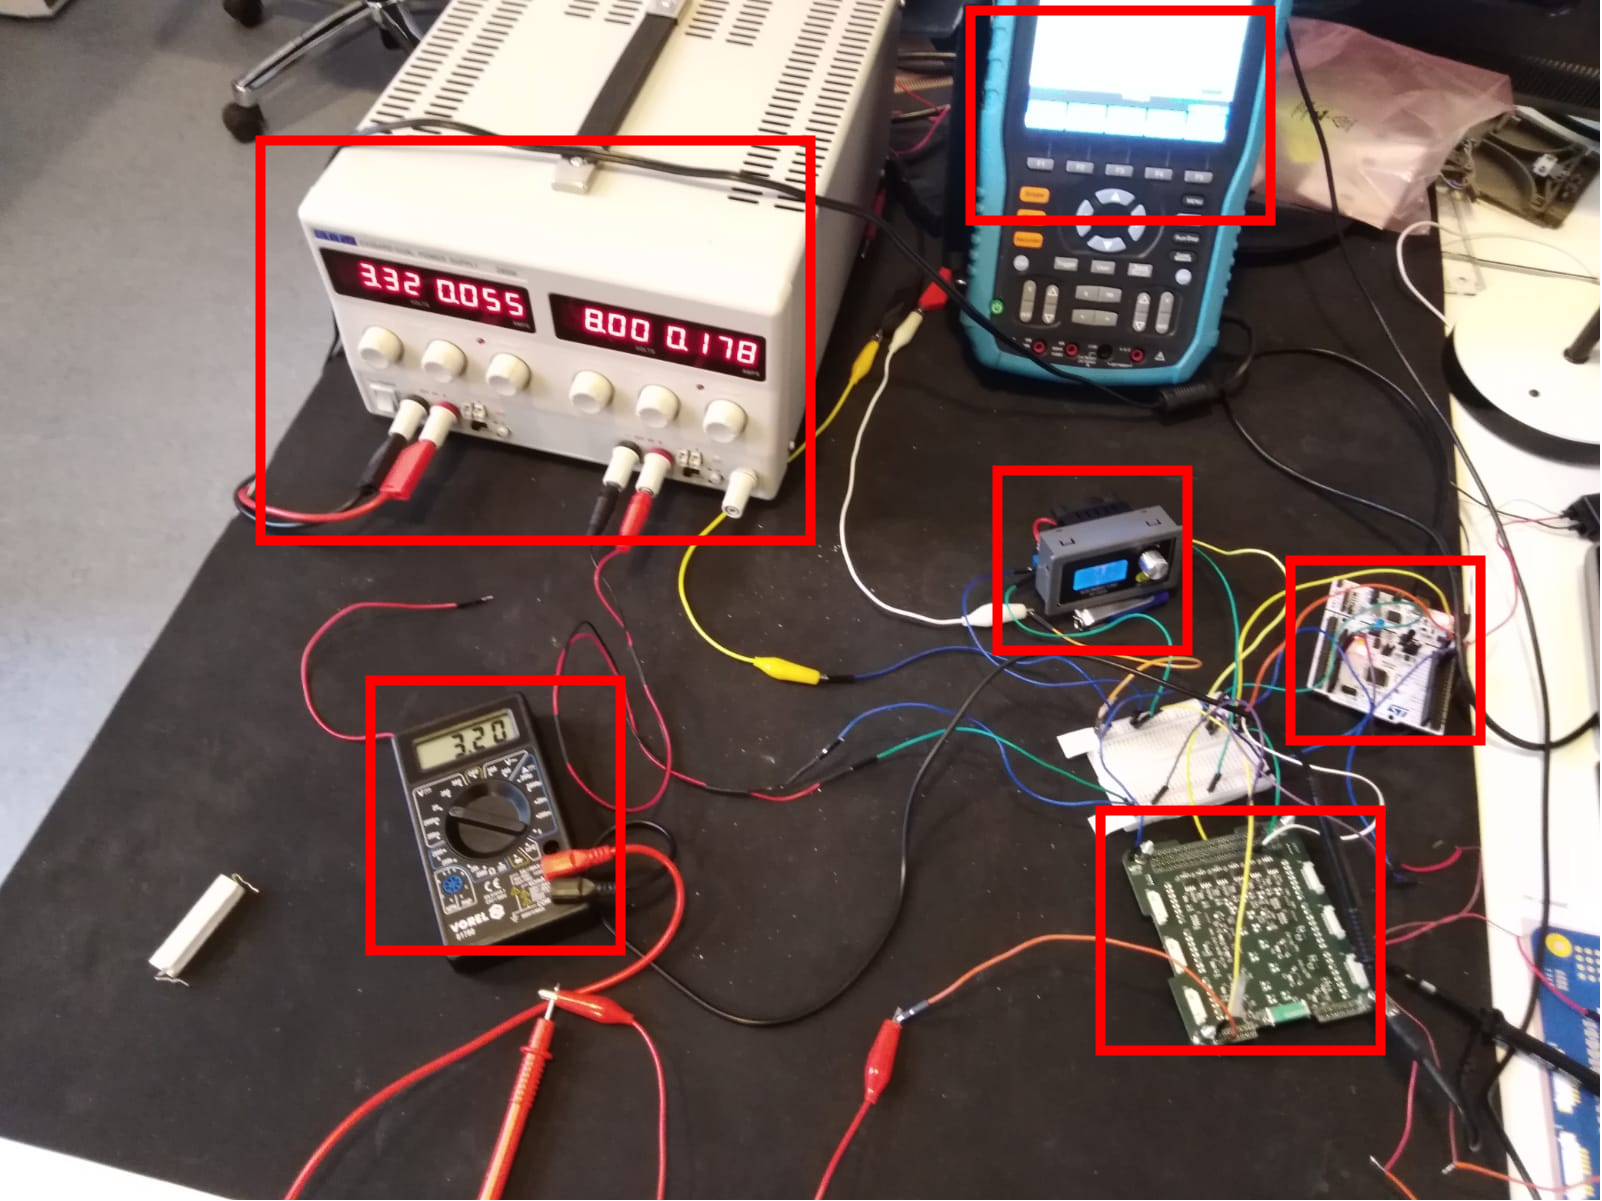
\includegraphics[scale=0.25]{pdu_test_tisch.png}
 	\caption{Load switches testbed}
 	\label{fig: pdu_test_tisch}
 \end{figure}

Figure \ref{fig: pdu_test_tisch} illustrates the switch test equipment used on the PDU. PSU supply 3.3V to the 3.3V BUS channel and 7.4V (the second PSU channel is not calibrated properly, to get 7.4V output it has to be adjusted for 8V). Testbed on the figure \ref{fig: pdu_test_tisch} is used to test DeCor payload of the VCC10 channel. In order to get all 7 steps done, shift register has to be switched off by sending a signal byte via microcontroller STM32. At the same time microcontroller used to provide an enable signal to the relative EN input pin of the PDU to activate the channel. Electical load is programed for 200$\mu$A to simulate the real load of DeCor. Multimeter on the picture connected to the $\overline{OC}$ pin with respect to the GND. With this configuration it is relatively easy to see the over-current condition of the PDU.\\ \\


 \begin{figure}[h]
 	\centering
 	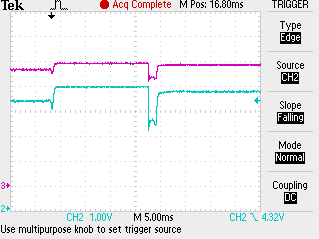
\includegraphics[scale=1.2]{hispico_plot.png}
 	\caption{Voltage drop of on the HISP power line in comparison with the 5V BUS voltage line}
 	\label{fig: oscilloscope}
 \end{figure}

Figure \ref{fig: oscilloscope} illustrates the voltage drop on the HISP line due to the inrush current of the Hispico S-band transceiver. The main issue of this voltage drop, is the Hispico input voltage tolerance, which is between 3.3V and 5V. The main challenge for the PDU is to keep voltage within the solution was reached by adding two capacitors into the output line that decrease the voltage drop. As shown on figure \ref{fig: oscilloscope} the maximum voltage drop on the HISP line (blue curve) reached 3.3V, which meets the requirements.

	
		
		Shift register check is done with help of microcontroller STM32 Nucleo -L073Rz. First of all I$^2$C line was adjusted by using CubeMX. After project was created, according to the datasheet of the shift register and section \ref{shiftty}, MAX7328 can be tested by sending a data to the port. This test was made by using HAL library.\\
		\begin{lstlisting}
		uint8_t val = 0x20; // value to send
		uint8_t slave = 0x1; // slave address
		HAL_I2C_Master_Transmit(&hi2c1,slave << 1,&val, 1, 100);
		\end{lstlisting}
	
	Upper mentioned code allows to enable the port P0 which sends the EN signal to the switch of VCC4 channel.
	
		\caption{Load switch test results}
		
		
		
		\begin{tabular}{p{2cm}p{2cm}p{2cm}p{2cm}p{2cm}p{2cm}}
			\toprule
			
			
			Channel & contact & VOUT output & OC contact & Curent max & Required current \\ \midrule
			VCC0 & pass & 3.3V & pass & 0.26A & 0.14A  \\ 
			VCC1 & pass & 3.3V & pass & 0.26A & 0.14A  \\ 
			VCC2 & pass & 5V & pass & 2A & 0.46A  \\ 
			VCC3 & pass & 3.3V & pass & 0,26 & 0.062A \\ 
			COM0 & pass & Vbat & pass & 2A & 0.69A  \\ 
			COM1 & pass & Vbat & pass & 2A & 0.69A  \\ 
			HISPICO & pass & 5V & pass & 2A & 1.5A \\ 
			VCC8 & pass & 5V & pass & 1.5A & 0.6A \\ 
			VCC9 & pass & 5V & pass & 0.26A & 0.04A \\ 
			VCC10 & pass & Vbat & pass & 0.27A & 0.04A \\ 
			VCC11 & pass & Vbat & pass & 0.27A & 0.2A \\ 
			VCC12 & pass & Vbat & pass & 0.27A & 0.04A \\ 
			VCC13 & pass & Vbat & pass & 0.27A & 0.2A \\ 
			VCC14 & pass & Vbat & pass & 0.27A & 0.04A \\ 
			VCC15 & pass & Vbat & pass & 0.27A & 0.2A \\ 
			VCC16 & pass & 5V & pass & 3A & 2A  \\ 
			VCC17 & pass & 5V & pass & 1.5A & 0.2A  \\ 
			VCC4 &  - &  - &  - &  - &  - \\ 
			VCC5 &  - &  - &  - &  - &  - \\ 
			VCC6 &  - &  - &  - &  - &  - \\ 
			VCC7 &  - &  - &  - &  - &  - \\ 
			VCC18 &  - &  - &  - &  - &  - \\ 
			VCC19 & pass & 5V & pass & 0.32A & 0.01A \\ 
			\bottomrule
		\end{tabular}
		\label{switchtest}\\
	
	Tab. \ref{switchtest} verifies top level requirements TL1-TL18.
	\section{Power Monitoring}
	
	To test the power monitoring of the PDU, the combination of ADC and Current sensors has to be tested. To accomplish this test, every power channel has to be tested separately by applying electrical load to each channel. \\
	
	STEPS:\\ \\
	\textbf{1.} First of all, Power Distribution Unit PCB has to be connected with a 3.3V BUS voltage to supply the ADC then, according to the power channel the needed voltage has to be also supplied. \\ \\
	\textbf{2.} After power  was supplied to the PCB, SPI signals has to be connected between PDU and a microcontroller STM32 Nucleo -L073Rz. SPI has a 3 signal lines: SLCK - clock line, MOSI - master output slave input and MISO - master input slave output. SPI protocol is a serial bus, to chose a slave SPI use the Slave select pin which is usually inverted. In the PDU board it has two slave select pins for each ADC.\\ \\
	\textbf{3.} After power and signal lines are connected, electric load can be added into the system by connecting it to the output pin of the relative channel.\\ \\
	\textbf{4.} The next step would be the reading current of the power line and displaying it on the monitor by using STM32 and minicom.
	  
	\begin{figure}[h]
		\centering
		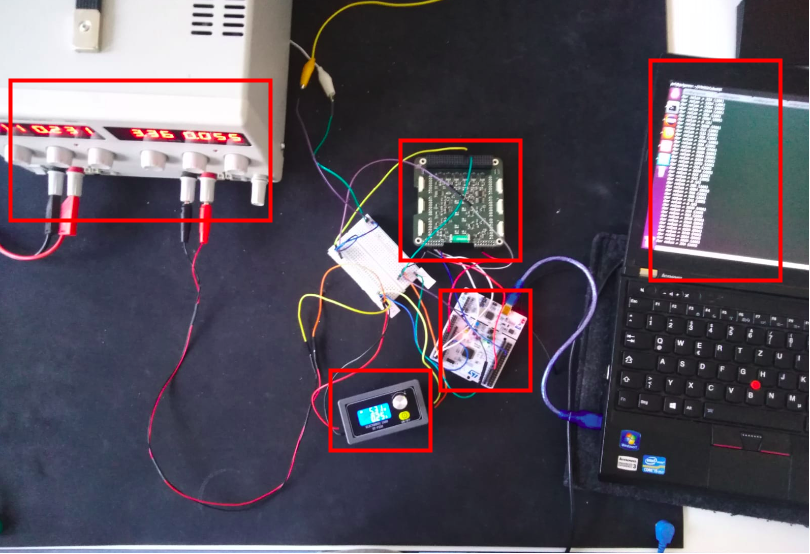
\includegraphics[scale=0.41]{adctest.png}
		\caption{Testbed of the Power monitoring test}
		\label{fig: adctest}
	\end{figure}
	 
	 To get the digital output values from the ADC, STM32 was adjusted and flashed with the following code:
	 
	
	 \begin{lstlisting}

	 uint8_t TxBuf[3];
	 uint8_t RxBuf[3];
	 uint8_t buffer[50];
	

	  while (1)
	  {
	  TxBuf[0] = 0x86;
	  TxBuf[1] = 0x0;
	  TxBuf[2] = 0x0;
	  HAL_GPIO_WritePin(GPIOA,GPIO_PIN_5, GPIO_PIN_RESET); //latch 
	  
	  HAL_SPI_TransmitReceive(&hspi2,TxBuf,RxBuf,3,100);
	  
	  
	  HAL_GPIO_WritePin(GPIOA,GPIO_PIN_5, GPIO_PIN_SET);
	  
	  uint8_t msb = RxBuf[1];
	  uint8_t lsb = RxBuf[2];
	  uint16_t VAL = ((uint16_t)msb << 8 | lsb) & 0x0FFF;
	  
	   int length = sprintf((char*)buffer, "Our value = %X \r\n",VAL);
	   
	   HAL_UART_Transmit(&huart2, buffer, length, 1000);
	   HAL_Delay(1000);
	   
	   }
	 \end{lstlisting}
	 
	 Upper mention code shows just the main variables and while loop, that was added in order to communicate with ADC. In addition, USART2 and SPI2 interfaces were adjusted via CubeMX.
	 
	 2nd to 4th line creating a buffers to store the data. According to the MAX1231 datasheet, to start converting process slave select pin (GPIO A5) has to be latched which is done on the 12th line.
	 Than to transmit the data via SPI master has to send 3 bytes, first should contain the information about the readable port and next two should be zeros, lines 9-11. This data is contained in the TxBuf buffer. To transmit and receive the data "HAL$\_$SPI$\_$TransmitReceive" command is used, line 14. After the transfer and receipt have been completed, RxBuf will contain two data bytes in RxBuf[1] - most significant byte and RxBuf[2] - less significant byte, lines 19, 20. GPIO pin has to latch down the slave select in order to finish the communication with the slave, line 17. After that, two bytes have to be merged into 16-bit variable, line 21. then the final value can be sent via UART to the computer, line 25.\\
	 After completing the test, for each power line, all 23 lines provided acceptable data which verifies the functional requirement FR3. Other requirements that shall be verified by the inspection have been successfully verified.
	 
	 
	 
		